\chapter{Deducción natural}

\section{Introducción}

En los anteriores capítulos hemos desarrollado unos sistemas formales fundamentados en semántica y valores de verdad, es decir, a cada fórmula le asociamos un valor de verdad, $V$ o $F$, que se puede obtener mediante interpretaciones. Sin embargo, si un objetivo de la lógica es formalizar razonamientos, nos interesa estudiar también un sistema formal centrado en cómo deducir unas proposiciones de otras, sin hacer falta la noción de verdad.\\

Por ejemplo, supongamos que queremos demostrar un teorema, que vendrá expresado por una fórmula $\psi$, y para deducirlo necesitamos unas fórmulas $\varphi_1,\varphi_2,\dots,\varphi_n$. Lo que queremos es una serie de reglas que nos digan cuándo una fórmula se deduce de otras, de modo que partiendo de unos axiomas y aplicando repetidamente estas reglas, podamos llegar en finitos pasos a que $\psi$ se deduce de $\varphi_1,\varphi_2,\dots,\varphi_n$.\\

De modo que nuestra intención ahora consiste en prestar atención a las \textit{reglas de inferencia}. Veremos a lo largo de este capítulo un sistema que solo conste de reglas de inferencia, así que comencemos por la siguiente


\begin{definition}
Una \textit{secuencia} es un par $\Gamma \idash \psi$ donde $\Gamma$ es un conjunto finito de fórmulas y $\psi$ es una fórmula que se denominan, respectivamente, \textit{conjunto de premisas} y \textit{conclusión}.
Normalmente, cuando $\Gamma$ es finito, denotamos la secuencia $\{\varphi_1, \dots, \varphi_n\} \idash \psi$ como $\varphi_1, \dots, \varphi_n \idash \psi$ y escribiremos $\Gamma, \varphi \idash \psi$ en vez de $\Gamma \cup \{\varphi\} \idash \psi$.
\end{definition}

Todas las reglas de nuestro sistema tendrán la forma:
\begin{prooftree}
\AxiomC{$\Gamma_1 \idash \varphi_1, \dots, \Gamma_n \idash \varphi_n$}
\UnaryInfC{$\Gamma \idash \varphi$}
\end{prooftree}
que intuitivamente significa: `se demuestra $\Gamma \idash \varphi$ si se demuestra cada secuencia $\Gamma_1 \idash \varphi_1, \dots, \Gamma_n \idash \varphi_n$'. \\[-5pt]

A lo largo de la exposición, veremos que existen reglas que no necesitan de premisas, que llamaremos \textit{axiomas}. En la siguiente sección exponemos las reglas y axiomas \textit{básicos}, y de ellos deduciremos después las reglas \textit{derivadas}.

\section{Reglas básicas}

\begin{itemize}
    \item[(\textbf{SP})] Axioma del supuesto: 
    \emph{si $\varphi\in\Gamma$, entonces $\Gamma\idash\varphi$ es un axioma.}
    
    \begin{center}
      \centerAlignProof
        (\textbf{SP})
      \quad
      \centerAlignProof
        \AxiomC{}
        \UnaryInfC{$\Gamma \idash \varphi$}
      \DisplayProof
      \quad
      \centerAlignProof
        $\varphi \in \Gamma$
    \end{center}
    

    \item[ (\textbf{FS})] Fortalecimiento del supuesto: 
    \emph{si $\Delta \idash \varphi$ y $\Gamma$ contiene a $\Delta$, se deduce $\Gamma \idash \varphi$.}
    \begin{center}
      \centerAlignProof
        (\textbf{FS})
      \quad
      \centerAlignProof
        \AxiomC{$\Delta \idash \varphi$}
        \UnaryInfC{$\Gamma \idash \varphi$}
      \DisplayProof
      \quad
      \centerAlignProof
        $\Delta \subseteq \Gamma$
    \end{center}

    \item[(\textbf{RC})] Razonamiento en cadena: 
    \emph{podemos demostrar un resultado intermedio $\psi$ y luego usarlo.}
\begin{prooftree}
\AxiomC{$\Gamma \idash \psi$}
\AxiomC{$\Gamma, \psi \idash \varphi$}
\BinaryInfC{$\Gamma \idash \varphi$}(\textbf{RC})
\end{prooftree}


    \item[ ($\land$\textbf{A})] Conjunción en el antecedente: 
    \begin{center}
      \centerAlignProof
        ($\land$\textbf{A})
      \quad
      \centerAlignProof
        \AxiomC{$\Gamma,\varphi,\psi \idash \chi$}
        \UnaryInfC{$\Gamma,\varphi\land\psi \idash \chi$}
      \DisplayProof
      \quad
      \centerAlignProof
    \end{center}


    \item[($\land$\textbf{C})] Conjunción en el consecuente.
\begin{prooftree}
\AxiomC{$\Gamma \idash \psi$}
\AxiomC{$\Gamma \idash \varphi$}
\BinaryInfC{$\Gamma \idash \psi \land \varphi$}($\land$\textbf{C})
\end{prooftree}

   \item[($\rightarrow \textbf{A}$)] Implicación en el antecedente: \emph{si tenemos una implicación
    en el antecedente, podemos intentar demostrar la premisa
    y entonces suponer el consecuente}.
  
  \begin{prooftree}
    \AxiomC{$\Gamma, \varphi \rightarrow \psi \idash \varphi$}
    \AxiomC{$\Gamma, \psi  \idash \chi$}
    \BinaryInfC{$\Gamma , \varphi \rightarrow \psi \idash \chi$}($\rightarrow \textbf{A}$)
   \end{prooftree}
   
   \item[($\rightarrow \textbf{C}$)] Implicación en el consecuente: \emph{ponemos el antecedente de la implicación en las premisas}.
   
   \begin{prooftree}
    \AxiomC{$\Gamma, \varphi \idash \psi$}
    \UnaryInfC{$\Gamma \idash \varphi \rightarrow \psi$}($\rightarrow \textbf{C}$)
   \end{prooftree}
   
   \item[($\lor \textbf{A}$)] Disyunción en el antecedente: \emph{si tenemos una distinción de casos hay que demostrar cada uno de los casos}.
   
   \begin{prooftree}
    \AxiomC{$\Gamma, \varphi \idash \chi$}
    \AxiomC{$\Gamma, \psi \idash \chi$}
    \BinaryInfC{$\Gamma, \varphi \lor\psi \idash \chi$}($\lor \textbf{A}$)
   \end{prooftree}
   
   \item[($\lor \textbf{C}_{1, 2}$)] Disyunción en el consecuente: \emph{basta demostrar uno de los elementos de la disyunción.} En realidad son dos reglas:
 
    \begin{center}
      \centerAlignProof
       ($\lor \textbf{C}_1$)
      \quad
      \centerAlignProof
        \AxiomC{$\Gamma \idash \varphi$}
        \UnaryInfC{$\Gamma \idash \varphi \lor \psi$}
      \DisplayProof
      \qquad
      \centerAlignProof
        ($\lor \textbf{C}_2$)
      \quad
      \centerAlignProof
      \AxiomC{$\Gamma \idash \psi$}
      \UnaryInfC{$\Gamma \idash \varphi \lor \psi$}
      \DisplayProof
    \end{center}
    
    \item[($\neg \textbf{A}$)] Negación en el antecedente.
   
   \begin{prooftree}
    \AxiomC{$\Gamma, \neg \varphi \idash \varphi$}
    \UnaryInfC{$\Gamma, \neg\varphi \idash \bot $}($\neg \textbf{A}$)
   \end{prooftree}
   
   \item[($\neg \textbf{C}$)] Negación en el consecuente.
   
   \begin{prooftree}
    \AxiomC{$\Gamma, \varphi \idash \bot$}
    \UnaryInfC{$\Gamma \idash \neg\varphi $}($\neg \textbf{C}$)
   \end{prooftree}
   
   \item[($\bot \textbf{A}$)] Axioma de contradicción en el antecente: \emph{si en el antecedente tenemos una contradicción podemos deducir cualquier cosa}.
 
   
   \begin{prooftree}
    \AxiomC{}
    \UnaryInfC{$\Gamma, \bot \idash \varphi $}($\bot \textbf{A}$)
   \end{prooftree}
   
   \item[(\textbf{DN}!)] Doble negación. 
   \begin{prooftree}
    \AxiomC{$\Gamma \idash \neg\neg\psi$}
    \UnaryInfC{$\Gamma \idash \psi $}(\textbf{DN}!)
   \end{prooftree}
   
   Esta regla se dice \emph{no constructiva}. La lógica intuicionista, por ejemplo, no la acepta.
   
   \item[($\forall \textbf{A}$)] Fórmula universal en el antecente: \emph{la fórmula universal se puede aplicar a cualquier término}.
   
   \begin{center}
      \centerAlignProof
        ($\forall \textbf{A}$)
      \quad
      \centerAlignProof
        \AxiomC{$\Gamma, \forall x \varphi, \varphi[t/x] \idash \psi$}
        \UnaryInfC{$\Gamma, \forall x \varphi \idash \psi $}
      \DisplayProof
      \quad
      \centerAlignProof
        $t\in TERM_{\overline{S}}$
    \end{center}
    
    \item[($\forall \textbf{C}*$)] Fórmula universal en el consecuente: \emph{demostramos la fórmula para un elemento genérico}.
   
   \begin{center}
      \centerAlignProof
        ($\forall \textbf{C}*$)
      \quad
      \centerAlignProof
        \AxiomC{$\Gamma \idash \varphi[c/x]$}
        \UnaryInfC{$\Gamma \idash \forall x \varphi $}
      \DisplayProof
      \quad
      \centerAlignProof
        $c\in C_A \text{  nueva}$
    \end{center}
    
    \item[($\exists \textbf{A}*$)] Fórmula existencial en el antecente: \emph{sabemos que existe un elemento que cumple la propiedad, lo nombramos}.
   
   \begin{center}
      \centerAlignProof
        ($\exists \textbf{A}*$)
      \quad
      \centerAlignProof
        \AxiomC{$\Gamma, \varphi[c/x] \idash \psi$}
        \UnaryInfC{$\Gamma, \exists x \varphi \idash \psi $}
      \DisplayProof
      \quad
      \centerAlignProof
        $c\in C_A \text{  nueva}$
    \end{center}
    
    \item[($\exists \textbf{C}$)] Fórmula existencial en el consecuente: \emph{basta encontrar un elemento que cumple la propiedad}.
    
    \begin{center}
      \centerAlignProof
        ($\exists \textbf{C}$)
      \quad
      \centerAlignProof
        \AxiomC{$\Gamma \idash \varphi[t/x]$}
        \UnaryInfC{$\Gamma \idash \exists x \varphi $}
      \DisplayProof
      \quad
      \centerAlignProof
        $t\in TERM_{\overline{S}}$
    \end{center}
    
    \item[ (\textbf{ID})] Axioma de identidad.
    
    \begin{center}
      \centerAlignProof
        (\textbf{ID})
      \quad
      \centerAlignProof
        \AxiomC{}
        \UnaryInfC{$\Gamma \idash t \doteq t $}
      \DisplayProof
      \quad
      \centerAlignProof
        $t\in TERM_{\overline{S}}$
    \end{center}
    
    \item[(\textbf{SUST})] Sustitución: \emph{si quiero demostrar la propiedad para un término t y sabemos que es igual a s, basta demostrar la propiedad para s}
    
    \begin{center}
      \centerAlignProof
        (\textbf{SUST})
      \quad
      \centerAlignProof
        \AxiomC{$\Gamma \idash \varphi[s/x]$}
        \UnaryInfC{$\Gamma, t\doteq s \idash \varphi[t/x] $}
      \DisplayProof
      \quad
      \centerAlignProof
        $t,s\in TERM_{\overline{S}}$
    \end{center}
\end{itemize}
    Las propiedades simétrica y transitiva pueden deducirse de esta regla.
    
\section{Árboles de deducción}

Una vez descritas las reglas básicas y dada una secuencia, para verificar si tal secuencia es o no correcta la descomponemos en las reglas básicas conocidas, es decir, revertimos la aplicación de las reglas básicas. La siguiente definición aclara estas nociones:
\begin{definition}
Un \textit{árbol de deducción} para una secuencia $\Gamma \idash \psi$ es un árbol de forma que nos nodos están etiquetados con secuencias, la raíz es $\Gamma \idash \psi$ y, dados un nodo $\Gamma_0 \idash \psi_0$ y sus hijos:
\begin{center}
\begin{tikzcd}
                                           & \Gamma_0 \idash \psi_0 \arrow[rd, no head] &                        \\
\Gamma_1 \idash \psi_1 \arrow[ru, no head] & \cdots                                 & \Gamma_n \idash \psi_n
\end{tikzcd}
\end{center}
se cumple que
\begin{prooftree}
\AxiomC{$\Gamma_0 \idash \psi_0 \quad \cdots \quad \Gamma_n \idash \psi_n$}
\UnaryInfC{$\Gamma \idash \psi$}
\end{prooftree}
es una regla.
\end{definition}

\begin{definition} \hspace{1} \\
\begin{enumerate}
    \item  Una secuencia $\Gamma \idash \psi$ se dice \textit{formalmente deducible}, $\vdash \Gamma \idash \psi$, si existe un árbol de deducción para $\Gamma \idash \psi$ con axiomas en las hojas. Si $\Gamma = \emptyset$, en vez de $\Gamma \idash \psi$ escribimos $\vdash \psi$.
    \begin{center}
    % https://tikzcd.yichuanshen.de/#N4Igdg9gJgpgziAXAbVABwnAlgFyxMJZARgBoAGAXVJADcBDAGwFcYkQAdDgcXoFs+9AARcsUenAAWIjmmwgAvqXSZc+QinKli1Ok1bsAggA98gxcpAZseAkTI6aDFm0QgAdJ4sqb6ogCZtXWcDNxMzekVdGCgAc3giUAAzACcIPiQtEBwIJDI9FyQwZkZGGkZ6ACMYRgAFVVsNEEYYJJwQGkkYeih2SDA2JWS0jMQsnKQAZid9V2LS8qqa+t87Nxa2jpAunr6CQctU9LyaCcRpkCksTcQAWkDt7t63fsHKBSA
    \begin{tikzcd}
                                             & \Gamma \idash \psi \arrow[ld, no head] \arrow[rd, no head] &        \\
    Axioma \arrow[rr, no head, shift left=2] & Axiomas                                                       & Axioma
    \end{tikzcd}
    \end{center}
    
    \item Si $\Phi$ es un conjunto de fórmulas (no necesariamente finito) diremos que una fórmula $\varphi$ es \emph{formalmente deducible a partir de $\Phi$}, y denotado por $\Phi \vdash \varphi$, si existe un subconjunto finito $\Gamma \subset \Phi$ tal que $\vdash \Gamma \idash \varphi$
\end{enumerate}
\end{definition}
$\Phi \vdash \varphi$ y $\vdash \Phi \idash \varphi$ son equivalentes si $\Phi$ es finito. $\Phi \vdash \varphi$ permite que $\Phi$ sea infinito y con $\vdash \Phi\idash \varphi$ se asume la finitud de $\Phi$. \\ \\
Veamos un primer ejemplo detallado de árbol de deducción:
\begin{example}\label{primerejemplo} \hspace{1} \\
\begin{center}
  \begin{tikzpicture}[sibling distance=5cm]
  \node (1) {\(\varphi\lor\psi,\neg\psi\idash\varphi\)}
  child{node (2) {\(\varphi,\neg\psi\idash \varphi\)}}
  child{
    node (3) {\(\psi,\neg\psi\idash \varphi\)}
    child{
      node{\(\psi,\neg\psi\idash \bot\)}
      child{
        node (5){\(\psi,\neg\psi\idash \psi\)}
        edge from parent node[right]{$\regla{\neg A}$}
      }
    }
    child{node (4){\(\psi,\neg\psi,\bot\idash \varphi\)}}
  };
  \node [below=1mm of 1] {\(\regla{\lor\mathbf{A}}\)};
  \node [below=1mm of 2] {\(\regla{SP}\)};
  \node [below=1mm of 3] {\(\regla{RC}\)};
  \node [below=1mm of 4] {\(\regla{\bot A}\)};
  \node [below=1mm of 5] {\(\regla{SP}\)};
\end{tikzpicture}
\end{center}
En este ejemplo, queremos llegar a que $\vdash \Gamma \idash \varphi$, siendo $\Gamma=\{\varphi\lor\psi,\neg\psi\}$. Como tenemos una disyunción en el antecedente, $\varphi\lor\psi$, podemos dividir por casos según la regla $\regla{\lor\mathbf{A}}$. \\
En una rama, tenemos $\varphi,\neg\psi\idash \varphi$. Como la conclusión es una premisa, esta secuencia es un axioma por ($\mathbf{SP}$).\\
En la otra rama, tenemos $\psi,\neg\psi\idash \varphi$. Está claro que $\psi,\neg\psi$ tiene que llevar a una contradicción, pero no hay ninguna regla que nos permita acabar directamente. En este caso podemos usar la regla ($\mathbf{RC}$), demostrando primero el resultado intermedio $\bot$ y luego demostrando $\varphi$ usando $\bot$. Esto lleva a una nueva división en ramas.\\
En la primera rama, tenemos $\psi,\neg\psi\idash\bot$. Como tenemos la fórmula $\neg\psi$ en el antecedente y $\bot$ en la conclusión, aplicamos la regla ($\neg\mathbf{A}$). Así, llegamos a la secuencia $\psi,\neg\psi\idash\psi$, que es un axioma ($\mathbf{SP}$).\\
En la segunda rama, tenemos $\psi,\neg\psi,\bot\idash\varphi$. Esta regla es un axioma ($\bot\mathbf{A}$), y hemos acabado.

\end{example}

\begin{example} \hspace{1} \\
    \begin{center}
  \begin{tikzpicture}
    \node{\(\forall x\, p(x)\rightarrow q(x)\quad \bigl(\forall x\,
      p(x)\bigr)\rightarrow\bigl(\forall x\,q(x)\bigr)\)}
    child{
      node{\(\forall x\, p(x)\rightarrow q(x),
        \forall x\,p(x)\quad \forall x\,q(x)\)}
      child {
        node{\(\forall x\, p(x)\rightarrow q(x),
          \forall x\,p(x)\quad q(c)\)}
        child {
          node{\(\forall x\, p(x)\rightarrow q(x),
            \forall x\,p(x),p(c)\rightarrow q(c)\quad q(c)\)}
          child {
            node{\(\forall x\, p(x)\rightarrow q(x),
              \forall x\,p(x),p(c)\rightarrow q(c), p(c)\quad q(c)\)}
            child [sibling distance=5cm]{
              node (1) {\(p(c)\rightarrow q(c), p(c)\quad q(c)\)}
              child{
                node(2){\(p(c)\rightarrow q(c), p(c)\quad p(c)\)}
              }
              child{
                node (3){\(p(c)\rightarrow q(c), q(c)\quad q(c)\)}
              }
              edge from parent node[right]{\(\regla{FS}\)}
            }
            edge from parent node[right]{\(\regla{\forall A}\)}
          }
          edge from parent node[right]{\(\regla{\forall A}\)}
        }
        edge from parent node[right]{\(\regla{\forall C*}\)}
      }
      edge from parent node[right]{\(\regla{\rightarrow C}\)}
    }
    ;
    \node[below=0mm of 1]{\(\regla{\rightarrow A}\)};
    \node[below=0mm of 2]{\(\regla{SP}\)};
    \node[below=0mm of 3]{\(\regla{SP}\)};
  \end{tikzpicture}
\end{center}

\end{example}

\section{Reglas derivadas}
Al crear árboles de deducción, hay una serie de razonamientos que se aplican muy frecuentemente pero que no vienen expresados por ninguna regla básica. Por ejemplo, en el ejemplo \ref{primerejemplo} para deducir la secuencia $\psi,\neg\psi\idash\varphi$, que parece tan obvia como un axioma, hemos necesitados tres nodos extra. Podemos resumir razonamientos frecuentes de este tipo en reglas que no son básicas pero se pueden deducir de ellas:

\begin{definition}
Una regla 
\begin{prooftree}
\AxiomC{$\Gamma_1 \idash \varphi_1 \quad \cdots \quad \Gamma_n \idash \varphi_n$}
\UnaryInfC{$\Gamma \idash \varphi$}
\end{prooftree}
con $n\geq0$ es derivable si existe un árbol de deducción para $\Gamma \idash \varphi$ cuyas hojas son axiomas o de la forma $\Gamma_i \idash \varphi_i,i=1,\dots,n$.
\end{definition}

Ahora, si tenemos un árbol de deducción $T$ para $\Gamma\idash\varphi$ que usa reglas básicas y derivadas, también existirá un árbol de deducción para $\Gamma\idash\varphi$ que solo usa reglas básicas. Informalmente, para obtener este nuevo árbol, basta con buscar en el árbol un nodo $\Gamma_0\idash\varphi_0$ que se ha obtenido de sus hijos mediante una regla derivada. De modo que fijándonos en ese nodo y sus hijos, el árbol será algo así:
\begin{center}
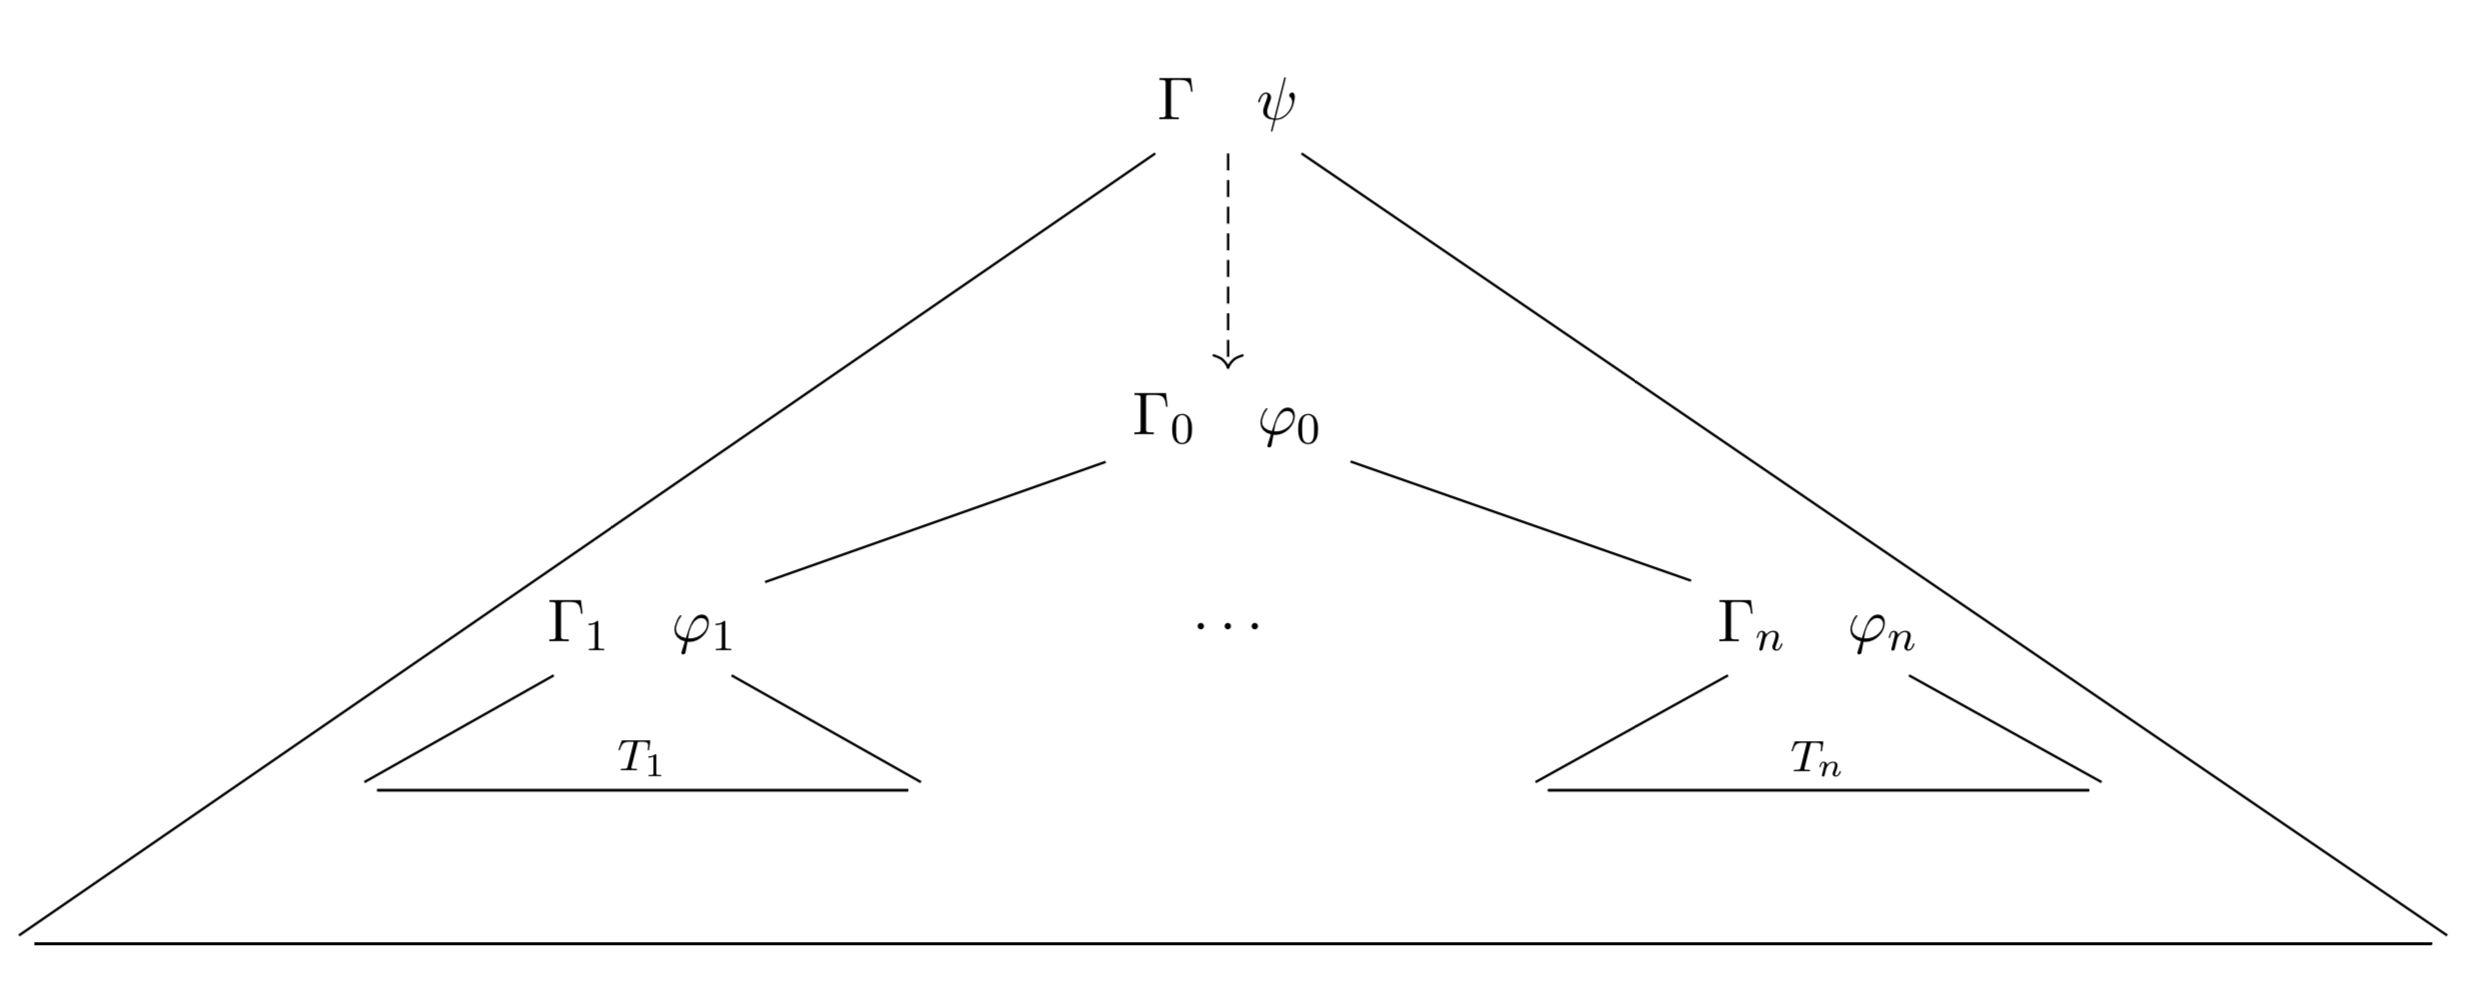
\includegraphics[scale = 0.3]{figures/arbol1.png}
% https://tikzcd.yichuanshen.de/#N4Igdg9gJgpgziAXAbVABwnAlgFyxMJZAVgBoAGAXVJADcBDAGwFcYkQAdDgcXoFs+9AARcsUenAAWIjmmwgAvqXSZc+QijIAmanSat2XXgPoB9cqPFSuDAE5pJWc4uUgM2PASIBmUt90MLGyInDz8gqYAjJYSkjb09o5RLioe6kQA7H4B+sGhxhFgMdYcdg5OhEqpal6a2TSBBiFcAMZQEDgIVW6qnhrIWqQALDlB7Ck9abXIQ8OjTSAT7jX9AGxzDbnj3ct9RAAcG3pjIUu96SjkpMTzeWdT-ZFXN5sniwq6MFAA5vBEoAAzWwQPhISI0HAQJBabpAkFgiFQxDeWHA0GIQYgSFIMggSQwehQdiQMBsVHwjGIpDrPEEokhElk1xw9G47GIGmMLCk9hwCBcok0fGE4kENgQ+hYRiink0Rj0ABGMEYAAVzrUQLYsN9JDgQDQpFgAXrEABaFHMtHUqmIXHC+ngMX6kCG41IXwgeVK1XqjSa7W652NPIAFWS5PRHvZWVpIoZToj7pth1jDsZExZSBj7JT9pl4pdjjdZotgKtiBT0aFdPzztdJo9XuVaoe7C1Or1rwWYcqlopVyxSPBICVYHpA65PJCVnxRMTiAH7IAnNW446efPF0OB3n4xu++iV4OwTua3uC-WkOb508bUfd+uL0WGx8FEA
\begin{comment}
\begin{tikzcd}
                               &  &                        &                                                                 &                                & \Gamma \quad \psi \arrow[dd, dashed] \arrow[lllllddddd, no head] \arrow[rrrrrddddd, no head] &                        &                                                                 &                                &  &                                \\
                               &  &                        &                                                                 &                                &                                                                                               &                        &                                                                 &                                &  &                                \\
                               &  &                        &                                                                 &                                & \Gamma_0\quad\varphi_0 \arrow[lld] \arrow[rrd]                                               &                        &                                                                 &                                &  &                                \\
                               &  &                        & \Gamma_1\quad\varphi_1 \arrow[ld, no head] \arrow[rd, no head] &                                & \cdots                                                                                        &                        & \Gamma_n\quad\varphi_n \arrow[ld, no head] \arrow[rd, no head] &                                &  &                                \\
                               &  & {} \arrow[rr, no head] &                                                                 & {} \arrow[ll, "A_1"', no head] &                                                                                               & {} \arrow[rr, no head] &                                                                 & {} \arrow[ll, "A_n"', no head] &  &                                \\
{} \arrow[rrrrrrrrrr, no head] &  &                        &                                                                 &                                &                                                                                               &                        &                                                                 &                                &  & {} \arrow[llllllllll, no head]
\end{tikzcd}
\end{comment}
\end{center}
donde $T_i$ es el árbol de deducción que se ha usado para llegar a $\Gamma_i\idash\varphi_i$. Ahora, simplemente, cambiamos el grafo formado por el nodo y sus $n$ hijos por el árbol de deducción de la regla derivada. Cuando en una hoja del árbol de la regla derivada aparece una secuencia $\Gamma_i\idash\varphi_i$, añadimos debajo de ella el árbol de deducción $T_i$. De modo que esquemáticamente obtenemos un árbol así:

\begin{center}
\begin{comment}
% https://tikzcd.yichuanshen.de/#N4Igdg9gJgpgziAXAbVABwnAlgFyxMJZAVgBoAGAXVJADcBDAGwFcYkQAdDgcXoFs+9AARcsUenAAWIjmmwgAvqXSZc+QijIAmanSat2XXgPoB9cqPFSuDAE5pJWc4uUgM2PASIBmUt90MLGyInDz8gqZYXACOzPRQNvT2jpEuKh7qRADsfgH6waHGEQBWMXEJHHYOTsVpbqqeGshapAAseUHsde5qXiitbR0GId0NmSgAbIM0gcMgoxl9yAAc03qdI0rpvU3kpMRDBQs7RACMewcz+V1b9YtNZP5XGyAAggAe+IIICrowUABzeBEUAAM1sED4SFONBwECQLRAkhg8XYkDAbBoUiwoJw0Nu4Mh0Nh8MQviRKKgaIImJA2NxSAAtKcCRCoYhEXCkAMKaiQui2KyiRySUgyLyqfyaXVCeyeVzEOLGFgMew4BBlVSaMi+eBpbD6FhGNTVTRGPQAEYwRgABTGfRAtiwAMkeKxjgZiHIQvZ4oVPJ1kr1prpHrxXrNlutdvu7CdLrd6zmABVUj6kOSFVMJSbacrVSF1ZqQAajbmSyBzVbbfaNI7na6ZWyM6LEDkc1LVenENmFe3A+X3Tjw97XLKkO2s9rKYPQ8OkHtK1Ga7GQvHG88U6Zat3FwqYSArWBJYv8wUrMiqbvW6sO8HBWPmxGQAqAJzT3UCpvC29vj9Br8h09UcwSfd8X1JW8B07Wl6RHbtOVJcloPvCs4KZbxu0zUlEXQsl-1nWYCmTCsq2jWs4wbPFfgUIA
\begin{tikzcd}
                               &  &                        &                                                                                                    &                                & \Gamma \idash \psi \arrow[dd, dashed] \arrow[lllllddddd, no head] \arrow[rrrrrddddd, no head] &                        &                                                                                                           &                                &  &                                \\
                               &  &                        &                                                                                                    &                                &                                                                                               &                        &                                                                                                           &                                &  &                                \\
                               &  &                        &                                                                                                    &                                & \Gamma_0\idash\varphi_0 \arrow[lld, no head, shift right] \arrow[rrd, no head, shift left]    &                        &                                                                                                           &                                &  &                                \\
                               &  &                        & \Gamma_i\quad\varphi_i \arrow[ld, no head] \arrow[rd, no head] \arrow[rrrr, no head, shift left=3] &                                & Axiomas                                                                                       &                       & \Gamma_j\quad\varphi_j \arrow[ld, no head] \arrow[rd, no head] \arrow[llll, "T"', no head, shift right=3] &                                &  &                                \\
                               &  & {} \arrow[rr, no head] &                                                                                                    & {} \arrow[ll, "T_i"', no head] &                                                                                               & {} \arrow[rr, no head] &                                                                                                           & {} \arrow[ll, "T_j"', no head] &  &                                \\
{} \arrow[rrrrrrrrrr, no head] &  &                        &                                                                                                    &                                &                                                                                               &                        &                                                                                                           &                                &  & {} \arrow[llllllllll, no head]
\end{tikzcd}
\end{comment}
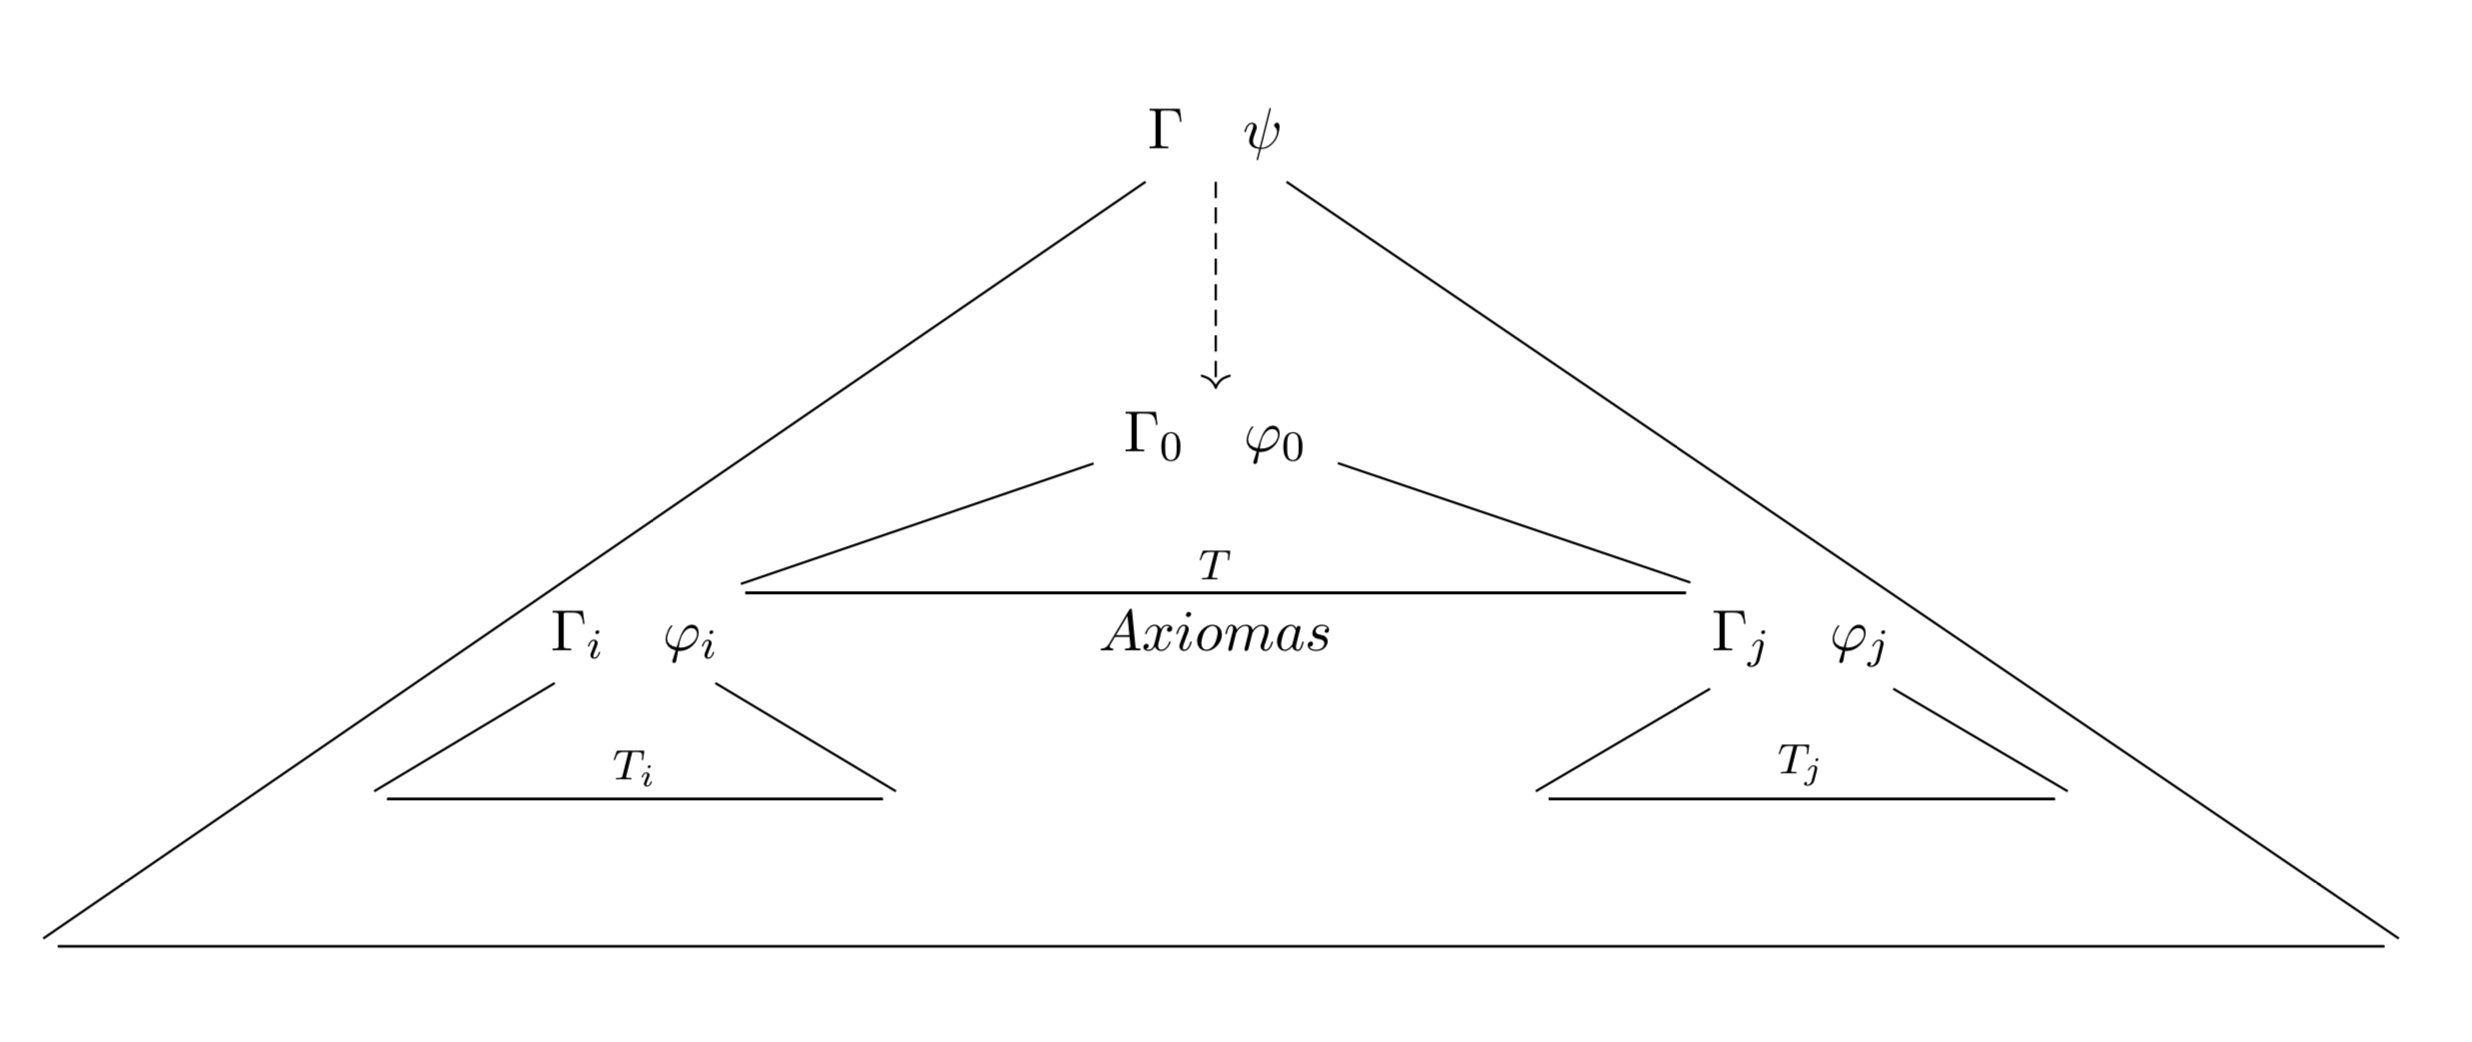
\includegraphics[scale = 0.3]{figures/arbol2.png}
\end{center}
donde en el árbol $T$ solo se usan reglas básicas y axiomas. Se puede demostrar que sustituyendo de este modo todas las reglas derivadas acabamos obteniendo un árbol en el que solo hay reglas básicas y axiomas.\\[10pt]
De modo que por lo que acabamos de ver, si tenemos un árbol para $\Gamma\idash\varphi$ que usa reglas básicas y derivadas, se cumple que $\Gamma\idash\varphi$ es formalmente deducible. Esto quiere decir que podemos usar sin problemas reglas derivadas que conocemos en los árboles de deducción.

\subsection{Repertorio de reglas derivadas}
En esta sección expondremos muchas reglas derivadas que permiten ver cómo razonamientos que hacemos habitualmente se expresan en el cálculo de secuencias. Para cada regla derivada incluímos su árbol de deducción.

\begin{itemize}
    \item Eliminación de una conjunción: \emph{siempre podemos demostrar un resultado más fuerte}. Son dos reglas simétricas.
    \begin{center}
      \centerAlignProof
       ($\textbf{E} \land$)
      \quad
      \centerAlignProof
        \AxiomC{$\Gamma \idash \psi\land\varphi$}
        \UnaryInfC{$\Gamma \idash \varphi $}
      \DisplayProof
      \qquad
      \centerAlignProof
        \AxiomC{$\Gamma \idash \varphi\land\psi$}
        \UnaryInfC{$\Gamma \idash \varphi $}
      \DisplayProof
    \end{center}
    \begin{proof} \hspace{1}
          \begin{center}
            \begin{tikzpicture}[sibling distance=5cm]
          \node (1) {\(\Gamma\idash \varphi\)}
              child{
                node (2){\(\Gamma\idash \psi\land\varphi\)}
              }
              child{
                node{\(\Gamma,\psi\land\varphi\idash \varphi\)}
                child{
                  node (3){\(\Gamma,\psi,\varphi\idash \varphi\)}
                  edge from parent node [right]{\(\regla{\land A}\)}
                }
              };
              \node[below=0mm of 1] {\(\regla{RC}\)};
              \node[below=0mm of 2] {Premisa};
              \node[below=0mm of 3] {\(\regla{SP}\)};
            \end{tikzpicture}
          \end{center}
    \end{proof}
    
    \item Modus Ponens
    \begin{center} 
      \centerAlignProof
       ($\textbf{MD}$)
      \quad
      \centerAlignProof
        \AxiomC{$\Gamma \idash \varphi \qquad \Gamma \idash \varphi \rightarrow \psi$}
        \UnaryInfC{$\Gamma \idash \psi $}
      \DisplayProof
    \end{center}
    \begin{proof} \hspace{1}
        \begin{center}
    \begin{tikzpicture}[sibling distance=5cm]
      \node (1){\(\Gamma\idash \psi\)}
      child{
        node (2){\(\Gamma\idash \varphi\)}
      }
      child{
        node (3){\(\Gamma,\varphi\idash \psi\)}
        child{
          node (4){\(\Gamma,\varphi,\varphi\rightarrow\psi\idash\psi\)}
          child{
            node
            (6){\(\Gamma,\varphi,\varphi\rightarrow\psi\idash\varphi\rightarrow\psi\)}
          }
          child{node (7){\(\Gamma,\psi\idash\psi\)}}
        }
        child{
          node {\(\Gamma,\varphi\idash\varphi\rightarrow\psi\)}
          child{
            node(5){\(\Gamma\idash\varphi\rightarrow\psi\)}
            edge from parent node[right]{\(\regla{FS}\)}
          }
        }
      };
      \node[below=0mm of 1] {\(\regla{RC}\)};
      \node[below=0mm of 2] {Premisa};
      \node[below=0mm of 3] {\(\regla{RC}\)};
      \node[below=0mm of 4] {\(\regla{\rightarrow A}\)};
      \node[below=0mm of 5] {Premisa};
      \node[below=0mm of 6] {Premisa};
      \node[below=0mm of 7] {Premisa};

    \end{tikzpicture}
  \end{center}
    \end{proof}
    \item Variante de la conjunción en el consecuente.
    \begin{center} 
      \centerAlignProof
       ($\land \textbf{C}'$)
      \quad
      \centerAlignProof
        \AxiomC{}
        \UnaryInfC{$\Gamma, \varphi, \psi \idash \varphi\land\psi $}
      \DisplayProof
    \end{center}
    \begin{proof} \hspace{1}
         \begin{center}
            \begin{tikzpicture}[sibling distance=5cm]
              \node (1){\(\Gamma,\varphi,\psi\idash \varphi\land\psi\)}
              child{
                node (2) {\(\Gamma,\varphi,\psi\idash \varphi\)}
              }
              child{
                node (3) {\(\Gamma,\varphi,\psi\idash \psi\)}
              };
              \node[below=0mm of 1]{\(\regla{\land C}\)};
              \node[below=0mm of 2]{\(\regla{SP}\)};
              \node[below=0mm of 3]{\(\regla{SP}\)};
            \end{tikzpicture}
          \end{center}
    \end{proof}
    
    \item Variante de la disyunción en el consecuente.
    \begin{center} 
      \centerAlignProof
       ($\lor \textbf{C}'$)
      \quad
      \centerAlignProof
        \AxiomC{}
        \UnaryInfC{$\Gamma, \varphi \idash \varphi\lor\psi $}
      \DisplayProof
      \quad
      \centerAlignProof
        \AxiomC{}
        \UnaryInfC{$\Gamma, \psi \idash \varphi\lor\psi $}
      \DisplayProof
    \end{center}
    \begin{proof} \hspace{1}
         \begin{center}
            \begin{tikzpicture}
              \node{\(\Gamma,\varphi\idash \varphi\lor\psi\)}
              child{
                node(1){\(\Gamma,\varphi\idash \varphi\)}
                edge from parent node[right]{\(\regla{\lor C}\)}
              }
              ;
              \node[below=0mm of 1]{\(\regla{SP}\)};
            \end{tikzpicture}
          \end{center}
    \end{proof}
    
    \item Reducción al absurdo: \emph{suponer la negación de la conclusión y llegar a una contradicción}.
    \begin{center} 
      \centerAlignProof
       ($\textbf{RA}!$)
      \quad
      \centerAlignProof
        \AxiomC{$\Gamma,\neg \varphi \idash \bot$}
        \UnaryInfC{$\Gamma \idash \varphi $}
      \DisplayProof
    \end{center}
    \begin{proof} \hspace{1}
        \begin{center}
        \begin{tikzpicture}
          \node{\(\Gamma\idash \varphi\)}
            child{
              node{\(\Gamma\idash \neg\neg\varphi\)}
              child{
                node (1){\(\Gamma,\neg\varphi\idash\bot\)}
                edge from parent node[right]{\(\regla{\neg C}\)}
              }
              edge from parent node[right]{\(\regla{DN!}\)}
            }
            ;
            \node[below=0mm of 1]{Premisa};
        \end{tikzpicture}
      \end{center}
    \end{proof}
    
    \item Reglas de la contradicción.
    \begin{center} 
      \centerAlignProof
       ($\textbf{CT}_1$)
      \quad
      \centerAlignProof
        \AxiomC{$\Gamma \idash \psi \qquad \Gamma \idash \neg\psi$}
        \UnaryInfC{$\Gamma \idash \varphi $}
      \DisplayProof
    \end{center}
    
    \begin{proof} \hspace{1}
        \begin{center}
        \begin{tikzpicture}[sibling distance=5cm]
          \node(0){\(\Gamma\idash \varphi\)}
            child{
              node(1){$\Gamma, \bot \idash \varphi$}
            }
            child{
              node(2){$\Gamma \idash \bot$}
              child{
                  node(3){$\Gamma, \neg \psi \idash \bot$}
                  child {
                        node(5){$\Gamma, \neg \psi \idash \psi$}
                        child {
                            node(6){$\Gamma\idash \psi$}
                            edge from parent node[right]{\(\regla{FS}\)}
                        }
                        edge from parent node[right]{\(\regla{\neg A}\)}
                  }
              }
              child{
                  node(4){$\Gamma \idash \neg \psi$}
              }
            }
            ;
            \node[below=0mm of 0]{(\textbf{RC})};
            \node[below=0mm of 1]{($\bot$ \textbf{A})};
            \node[below=0mm of 2]{(\textbf{RC})};
            \node[below=0mm of 4]{Premisa};
            \node[below=0mm of 6]{Premisa};
        \end{tikzpicture}
      \end{center}
    \end{proof}
    
    \begin{center} 
      \centerAlignProof
       ($\textbf{CT}_2$)
      \quad
      \centerAlignProof
        \AxiomC{}
        \UnaryInfC{$\Gamma, \varphi, \neg\varphi \idash \psi $}
      \DisplayProof
    \end{center}
    
        \begin{proof} \hspace{1}
        \begin{center}
        \begin{tikzpicture}[sibling distance=4cm]
            \node(0){$\Gamma, \varphi, \neg\varphi \idash \psi$}
            child {
                node(1){$\Gamma, \varphi, \neg \varphi, \idash \neg \varphi$}
            }
            child {
                node(2){$\Gamma, \varphi, \neg \varphi, \idash \varphi$}
            }
            ;
            \node[below=0mm of 0]{($\textbf{CT}_1$)};
            \node[below=0mm of 1]{(\textbf{SP})};
            \node[below=0mm of 2]{(\textbf{SP})};
        \end{tikzpicture}
      \end{center}
      
      
    \end{proof}
    \item  Reglas de la doble negación.
    
    \begin{center} 
      \centerAlignProof
       ($\neg\neg\textbf{C}$)
      \quad
      \centerAlignProof
        \AxiomC{$\Gamma \idash \varphi$}
        \UnaryInfC{$\Gamma \idash \neg\neg\varphi $}
      \DisplayProof
      \qquad 
      \centerAlignProof
       ($\neg\neg\textbf{A}!$)
      \quad
      \centerAlignProof
        \AxiomC{$\Gamma,\varphi\idash \psi$}
        \UnaryInfC{$\Gamma,\neg\neg\varphi\idash \psi$}
      \DisplayProof
    \end{center}
    
    \begin{proof} \hspace{1}
        \begin{center}
        \begin{tikzpicture}[sibling distance=4cm]
            \node(0){$\Gamma \idash \neg\neg\varphi$}
            child{
                node(1){$\Gamma\idash \varphi$}
            }
            child {
                node(2){$\Gamma,\varphi \idash \neg\neg \varphi$}
                child {
                    node(3) {$\Gamma,\varphi,\neg\varphi \idash \bot$}
                    edge from parent node[right]{\(\regla{\neg C}\)}
                }
            }
            ;
            \node[below=0mm of 0]{($\textbf{RC}$)};
            \node[below=0mm of 1]{Premisa};
            \node[below=0mm of 3]{($\textbf{CT}_2$)};
        \end{tikzpicture}
        \end{center}
        \begin{center}
        \begin{tikzpicture}[sibling distance=4cm]
            \node(0){$\Gamma,\neg\neg\varphi\idash \psi$}
            child{
                node(1){$\Gamma,\neg\neg\varphi\idash \varphi$}
                child {
                    node(3){$\Gamma,\neg\neg\varphi \idash \neg\neg\varphi$}
                    edge from parent node[right]{\(\regla{DN!}\)}
                }
            }
            child {
                node(2){$\Gamma,\neg\neg\varphi,\varphi \idash \psi$}
                child {
                    node(4){$\Gamma,\varphi \idash \psi$}
                    edge from parent node[right]{\(\regla{FS}\)}
                }
            }
            ;
            \node[below=0mm of 0]{($\textbf{RC}$)};
            \node[below=0mm of 3]{($\textbf{SP}$)};
            \node[below=0mm of 4]{Premisa};
        \end{tikzpicture}
      \end{center}
      
    \end{proof}
    
    \item  Reglas de la contraposición.
    
    \begin{center} 
      \centerAlignProof
       ($\textbf{CP}_1$)
      \quad
      \centerAlignProof
        \AxiomC{$\Gamma,\psi \idash \varphi$}
        \UnaryInfC{$\Gamma,\neg \varphi \idash \neg\psi $}
      \DisplayProof
      \qquad 
      \centerAlignProof
       ($\textbf{CP}_2$)
      \quad
      \centerAlignProof
        \AxiomC{$\Gamma,\varphi \idash \neg\psi $}
        \UnaryInfC{$\Gamma,\psi \idash \neg\phi$}
      \DisplayProof
    \end{center}
    
    \begin{proof} \hspace{1}
        \begin{center}
        \begin{tikzpicture}[sibling distance=4cm]
            \node(0) {$\Gamma,\neg\varphi \idash \neg\psi$}
            child {
                node(1){$\Gamma, \neg\varphi, \psi \idash \bot$}
                child {
                    node(2){$\Gamma, \neg\varphi, \psi \idash \varphi$}
                    child {
                        node(4){$\Gamma, \psi \idash \varphi$}
                        edge from parent node[right]{($\textbf{SP}$)}
                    }
                }
                child {
                    node(3){$\Gamma, \neg\varphi, \psi, \varphi \idash \bot$}
                }
                edge from parent node[right]{($\neg\textbf{C}$)}
            }
            ;
             \node[below=0mm of 1]{($\textbf{RC}$)};
             \node[below=0mm of 3]{($\textbf{CT}_2$)};
             \node[below=0mm of 4]{Premisa};
        \end{tikzpicture}
        \end{center}
        
    \end{proof}
    
    \begin{center} 
      \centerAlignProof
       ($\textbf{CP}_3$)
      \quad
      \centerAlignProof
        \AxiomC{$\Gamma,\neg\varphi \idash \neg\psi$}
        \UnaryInfC{$\Gamma,\psi \idash \varphi $}
      \DisplayProof
      \qquad 
      \centerAlignProof
       ($\textbf{CP}_4$)
      \quad
      \centerAlignProof
        \AxiomC{$\Gamma,\neg\varphi \idash \psi$}
        \UnaryInfC{$\Gamma,\neg\psi \idash \varphi $}
      \DisplayProof
    \end{center}
    \begin{proof} \hspace{1}
        \begin{center}
        \begin{tikzpicture}[sibling distance=4cm]
            \node(0) {$\Gamma,\psi \idash \varphi$}
            child {
                node(1){$\Gamma, \psi \idash \neg\neg\varphi$}
                child {
                    node(2){$\Gamma, \neg\varphi \idash \neg\psi$}
                    edge from parent node[right]{($\textbf{CP}_2$)}
                }
                edge from parent node[right]{($\textbf{DN}!$)}
            }
            ;
            \node[below=0mm of 2]{Premisa};
        \end{tikzpicture}
        \end{center}
        
    \end{proof}
    
    \item  Otras reglas no constructivas.
    
    \begin{center} 
      \centerAlignProof
       ($\textbf{VC}!$)
      \quad
      \centerAlignProof
        \AxiomC{$\Gamma,\neg\varphi \idash \psi$}
        \UnaryInfC{$\Gamma\idash \varphi \lor\psi $}
      \DisplayProof
      \qquad 
      \centerAlignProof
        \AxiomC{$\Gamma,\neg\psi \idash \varphi$}
        \UnaryInfC{$\Gamma\idash \varphi \lor\psi $}
      \DisplayProof
    \end{center}
    
    \begin{proof} \hspace{1}
        \begin{center}
        \begin{tikzpicture}[sibling distance=4cm]
            \node(0) {$\Gamma\idash \varphi \lor\psi$}
            child {
                node(1) {$\Gamma, \neg(\varphi\lor \psi)\idash \bot$}
                child {
                    node(2) {$\Gamma, \neg(\varphi\lor \psi)\idash \varphi\lor \psi$}
                    child {
                        node(3) {$\Gamma, \neg(\varphi\lor \psi)\idash \varphi$}
                        child {
                            node(4) {$\Gamma, \neg \varphi \idash \varphi\lor\psi$}
                            child {
                                node(5){$\Gamma, \neg\varphi\idash \psi$}
                                edge from parent node [right]{($\lor\textbf{C}$)}
                            }
                            edge from parent node [right]{($\textbf{CP}_4$)}
                        }
                        edge from parent node[right]{($\lor\textbf{C}$)}
                    }
                    edge from parent node[right]{($\neg\textbf{A}$)}
                }
                edge from parent node[right]{($\textbf{RA}!$)}
            }
            
            ;
            \node[below=0mm of 5]{Premisa};
        \end{tikzpicture}
        \end{center}
    \end{proof}
    
    \begin{center} 
      \centerAlignProof
       ($\textbf{TE}!$)
      \quad
      \centerAlignProof
        Tercio excluido
      \qquad 
      \centerAlignProof
        \AxiomC{}
        \UnaryInfC{$\Gamma\idash \varphi \lor\neg\varphi $}
      \DisplayProof
    \end{center}
     \begin{proof} \hspace{1}
        \begin{center}
        \begin{tikzpicture}[sibling distance=4cm]
            \node(0) {$\Gamma\idash \varphi \lor\neg\varphi$}
            child {
                node(1) {$\Gamma, \neg\varphi \idash \neg\varphi$}
                edge from parent node[right]{($\textbf{VC}!$)}
            }
            
            ;
            \node[below=0mm of 1]{($\textbf{SP}$)};
        \end{tikzpicture}
        \end{center}
    \end{proof}
    
    \begin{center} 
      \centerAlignProof
       ($\textbf{DC}!$)
      \quad
      \centerAlignProof
        Distinción de casos
      \qquad 
      \centerAlignProof
        \AxiomC{$\Gamma, \varphi\idash \psi\qquad \Gamma, \neg\varphi\idash \psi$}
        \UnaryInfC{$\Gamma\idash \psi$}
      \DisplayProof
    \end{center}
    \begin{proof} \hspace{1}
        \begin{center}
        \begin{tikzpicture}[sibling distance=4cm]
            \node(0) {$\Gamma\idash \psi$}
            child {
                node(1) {$\Gamma \idash \varphi\lor\neg\varphi$}
            }
            child {
                node(2) {$\Gamma,\varphi\lor\neg\varphi \idash \psi$}
                child {
                    node(3) {$\Gamma, \varphi \idash \psi$}
                }
                child {
                    node(4) {$\Gamma, \neg\varphi \idash \psi$}
                }
            }
            ;
            \node[below=0mm of 0]{($\textbf{RC}$)};
            \node[below=0mm of 1]{($\textbf{TE}$!)};
            \node[below=0mm of 2]{($\lor\textbf{A}$!)};
            \node[below=0mm of 3]{Premisa};
            \node[below=0mm of 4]{Premisa};
        \end{tikzpicture}
        \end{center}
    \end{proof}
    
    \begin{center} 
      \centerAlignProof
       ($\rightarrow\textbf{A}!$)
      \quad
      \qquad 
      \centerAlignProof
        \AxiomC{$\Gamma, \neg \varphi  \idash \chi \qquad \Gamma, \psi  \idash \chi$}
        \UnaryInfC{$\Gamma, \varphi \rightarrow \psi \idash \chi$}
      \DisplayProof
    \end{center}
    \begin{proof} \hspace{1}
        \begin{center}
            \begin{tikzpicture}[sibling distance=5cm]
                \node(0) {$\Gamma, \varphi \rightarrow \psi \idash \chi$}
                child {
                    node(1) {$\Gamma, \neg \varphi, \varphi \rightarrow\psi \idash \chi$}
                    child {
                        node(3) {$\Gamma, \neg \varphi \idash \chi$}
                        edge from parent node[right]{($\textbf{FS}$)}
                    }
                }
                child {
                    node(2) {$\Gamma, \varphi, \varphi \rightarrow\psi \idash \chi$}
                    child {
                        node(4) {$\Gamma, \varphi, \varphi\rightarrow \psi \idash \varphi$}
                    }
                    child {
                        node(5) {$\Gamma, \varphi, \psi \idash \chi$}
                        child {
                            node(6){$\Gamma,\psi \idash \chi$}
                            edge from parent node[right]{($\textbf{FS}$)}
                        }
                    }
                }
                ;
                \node[below=0mm of 0]{($\textbf{DC}$!)};
                \node[below=0mm of 2]{($\rightarrow\textbf{A}$)};
                \node[below=0mm of 3]{Premisa};
                \node[below=0mm of 4]{($\textbf{SP}$)};
                \node[below=0mm of 6]{Premisa};
            \end{tikzpicture}
        \end{center}
    \end{proof}
\end{itemize}

(PENDIENTE DE ACABAR)


\section{Corrección}

Ya hemos definido anteriormente lo que significa que $\varphi$ sea formalmente deducible a partir de $\Phi$, $\Phi\vdash\varphi$. Vamos a comparar ahora esto con la semántica que hemos visto en el tema anterior.\\


Para que la deducción natural sea compatible con la semántica, nos interesa ver que $\Phi$ implica $\varphi$ si y solo si $\varphi$ es formalmente deducible a partir de $\Phi$. Expresándolo formalmente, queremos ver que $\Gamma\vDash\varphi$ si y solo si $\Gamma\vdash\varphi$. Esto se divide en dos implicaciones:

\begin{itemize}
    \item Corrección: $\Phi\vdash\varphi$ implica $\Phi\vDash\varphi$.
    \item Completitud: $\Phi\vDash\varphi$  implica $\Phi\vdash\varphi$.
\end{itemize}

En esta sección se demostrará la corrección de la deducción natural, y la siguiente sección se dedicará a la completitud.\\[10pt]
\begin{definition}
Diremos que una secuencia $\Gamma\idash\varphi$ es \textit{correcta} si se cumple $\Gamma\vDash\varphi$. Es decir, informalmente, si `las premisas implican la conclusión'.
\end{definition}

\begin{definition}
Una regla 
\begin{prooftree}
\AxiomC{$\Gamma_1 \idash \varphi_1, \dots, \Gamma_n \idash \varphi_n$}
\UnaryInfC{$\Gamma \idash \varphi$}
\end{prooftree}
se dice \textit{correcta} si la secuencia $\;\Gamma \idash \varphi\;$ es correcta siempre que lo sean  $\;\Gamma_1 \idash \varphi_1, \dots, \Gamma_n \idash \varphi_n$. Es decir, si se cumplen $\Gamma_1\vDash\varphi_1,\dots,\Gamma_n\vDash\varphi_n$, entonces se cumple $\Gamma\vDash\varphi$.
\end{definition}

Conviene hacer notar que un axioma 
\begin{prooftree}
\AxiomC{}
\UnaryInfC{$\Gamma \idash \varphi$}
\end{prooftree}
es correcto si $\Gamma \vDash \varphi$.

\begin{prop}
Todas las reglas y axiomas básicos son correctos.
\end{prop}
\begin{proof}
Se comprueba directamente. Haremos algunas demostraciones a modo de ejemplo.
\begin{prooftree}
\AxiomC{$\Gamma \idash \psi$}
\AxiomC{$\Gamma, \psi \idash \varphi$}
\BinaryInfC{$\Gamma \idash \varphi$}(\textbf{RC})
\end{prooftree}
Supongamos que $\Gamma \vDash \psi$, $\Gamma, \psi \vDash \varphi$. Sea una interpretación $\mathfrak{I}$ tal que $\mathfrak{I} \vDash \Gamma$. Al ser $\Gamma \vDash \psi$, $\mathfrak{I} \vDash \psi$ y por tanto $\mathfrak{I} \vDash \Gamma \cup \{\psi\}$, y como $\Gamma, \psi \vDash \varphi$, $\mathfrak{I} \vDash \varphi$. Como esto lo cumple cualquier modelo $\mathfrak{I}$, tenemos que $\Gamma \vDash \varphi$.
\\
 \begin{prooftree}
    \AxiomC{$\Gamma, \varphi \rightarrow \psi \idash \varphi$}
    \AxiomC{$\Gamma, \psi  \idash \chi$}
    \BinaryInfC{$\Gamma , \varphi \rightarrow \psi \idash \chi$}($\rightarrow \textbf{A}$)
  \end{prooftree}
Supongamos que $\Gamma, \varphi \rightarrow \psi \vDash \varphi$, $\Gamma, \psi  \vDash \chi$. Sea $\mathfrak{I}$ tal que $\mathfrak{I}\vDash \Gamma, \varphi \rightarrow \psi$. Por tanto, $\mathfrak{I} \vDash \varphi$ y $\mathfrak{I} \vDash \varphi \rightarrow \psi$, es decir, $\mathfrak{I} \vDash \psi$. Por otro lado, como también $\mathfrak{I} \vDash \Gamma$, entonces $\mathfrak{I} \vDash \Gamma \cup \{\psi\}$, con lo que $\mathfrak{I} \vDash \chi$. Al ser $\mathfrak{I}$ arbitrario, $\Gamma \cup \{\varphi \rightarrow \psi\} \vDash \chi$.
\\
\begin{center}
      \centerAlignProof
        ($\forall \textbf{A}$)
      \quad
      \centerAlignProof
        \AxiomC{$\Gamma, \forall x \varphi, \varphi[t/x] \idash \psi$}
        \UnaryInfC{$\Gamma, \forall x \varphi \idash \psi $}
      \DisplayProof
      \quad
      \centerAlignProof
        $t\in TERM_{\overline{S}}$
    \end{center}
Sea $\mathfrak{I} \vDash \Gamma \cup \{\forall x \, \varphi\}$. Entonces, para todo $a \in A$ (con $A$ conjunto soporte de $\mathfrak{I}$), $\mathfrak{I}[a/x] \vDash \varphi$ y, por ser $t^{\mathfrak{I}} \in A$, tenemos que $\mathfrak{I}[t^{\mathfrak{I}}/x]\vDash \varphi$. Por el Lema de Sustitución, $\mathfrak{I} \vDash \varphi[t/x]$. Por tanto, $\mathfrak{I} \vDash \Gamma \cup \{\forall x \, \varphi, \varphi[t/x]\}$ y, como suponemos que $\Gamma, \forall x \, \varphi, \varphi[t/x] \vDash \psi$, obtenemos que $\mathfrak{I} \vDash \psi$, lo que nos da el resultado.
\end{proof}